\documentclass{beamer}
\mode<presentation>
\usepackage{amsmath}
\usepackage{amssymb}
%\usepackage{advdate}
\usepackage{adjustbox}
\usepackage{subcaption}
\usepackage{enumitem}
\usepackage{multicol}
\usepackage{mathtools}
\usepackage{listings}
\usepackage{float}
\usepackage{graphicx}
\usepackage{url}
\def\UrlBreaks{\do\/\do-}
\usetheme{Boadilla}
\usecolortheme{lily}
\setbeamertemplate{footline}
{
  \leavevmode%
  \hbox{%
  \begin{beamercolorbox}[wd=\paperwidth,ht=2.25ex,dp=1ex,right]{author in head/foot}%
    \insertframenumber{} / \inserttotalframenumber\hspace*{2ex} 
  \end{beamercolorbox}}%
  \vskip0pt%
}
\setbeamertemplate{navigation symbols}{}

\providecommand{\nCr}[2]{\,^{#1}C_{#2}} % nCr
\providecommand{\nPr}[2]{\,^{#1}P_{#2}} % nPr
\providecommand{\mbf}{\mathbf}
\providecommand{\pr}[1]{\ensuremath{\Pr\left(#1\right)}}
\providecommand{\qfunc}[1]{\ensuremath{Q\left(#1\right)}}
\providecommand{\sbrak}[1]{\ensuremath{{}\left[#1\right]}}
\providecommand{\lsbrak}[1]{\ensuremath{{}\left[#1\right.}}
\providecommand{\rsbrak}[1]{\ensuremath{{}\left.#1\right]}}
\providecommand{\brak}[1]{\ensuremath{\left(#1\right)}}
\providecommand{\lbrak}[1]{\ensuremath{\left(#1\right.}}
\providecommand{\rbrak}[1]{\ensuremath{\left.#1\right)}}
\providecommand{\cbrak}[1]{\ensuremath{\left\{#1\right\}}}
\providecommand{\lcbrak}[1]{\ensuremath{\left\{#1\right.}}
\providecommand{\rcbrak}[1]{\ensuremath{\left.#1\right\}}}
\theoremstyle{remark}
\newtheorem{rem}{Remark}
\newcommand{\sgn}{\mathop{\mathrm{sgn}}}
\providecommand{\abs}[1]{\left\vert#1\right\vert}
\providecommand{\res}[1]{\Res\displaylimits_{#1}} 
\providecommand{\norm}[1]{\lVert#1\rVert}
\providecommand{\mtx}[1]{\mathbf{#1}}
\providecommand{\mean}[1]{E\left[ #1 \right]}
\providecommand{\fourier}{\overset{\mathcal{F}}{ \rightleftharpoons}}
%\providecommand{\hilbert}{\overset{\mathcal{H}}{ \rightleftharpoons}}
\providecommand{\system}{\overset{\mathcal{H}}{ \longleftrightarrow}}
	%\newcommand{\solution}[2]{\textbf{Solution:}{#1}}
%\newcommand{\solution}{\noindent \textbf{Solution: }}
\providecommand{\dec}[2]{\ensuremath{\overset{#1}{\underset{#2}{\gtrless}}}}
\newcommand{\myvec}[1]{\ensuremath{\begin{pmatrix}#1\end{pmatrix}}}
\let\vec\mathbf

\lstset{
language=C,
frame=single, 
breaklines=true,
columns=fullflexible
}

\numberwithin{equation}{section}

\title{Presentation - Matgeo}
\author{Aryansingh Sonaye \\
AI25BTECH11032 \\
EE1030 - Matrix Theory}

\date{\today} 
\begin{document}

\begin{frame}
\titlepage
\end{frame}

\section{Problem}
\begin{frame}
\frametitle{Problem Statement}
\textbf{Problem Statement}

Find the equation of the plane passing through the intersection of the planes 
\begin{align}
\vec{n}_1^\top \vec{x} - c_1 = 0, 
\qquad
\vec{n}_2^\top \vec{x} - c_2 = 0
\end{align}

which is parallel to the $x$-axis, and compute the perpendicular distance of this plane from the $x$-axis.

\end{frame}

\section{Solution}
\subsection{Description of Variables used}
\begin{frame}
\frametitle{Description of Variables used}
\begin{table}[H]
\centering
\begin{tabular}{|c|c|}
\hline
\textbf{Quantity} & \textbf{Value} \\
\hline
$\vec{n}_1$ & $\myvec{1\\1\\1}$ \\
\hline
$c_1$ & $1$ \\
\hline
$\vec{n}_2$ & $\myvec{2\\3\\-1}$ \\
\hline
$c_2$ & $-4$ \\
\hline
$\vec{e}_1$ & $\myvec{1\\0\\0}$ \\
\hline
\end{tabular}
\caption{Input data for the problem}
\label{}
\end{table}


\end{frame}

\subsection{Theoretical Solution }
\begin{frame}
\frametitle{Theoretical Solution}
\textbf{Step 1. General plane through the intersection}
\begin{align}
\big(\vec{n}_1 + k \vec{n}_2\big)^\top \vec{x} - \big(c_1 + k c_2\big) &= 0 \\
\vec{n} &= \vec{n}_1 + k \vec{n}_2 \\
c &= c_1 + k c_2
\end{align}

\textbf{Step 2. Condition for parallelism with $x$-axis}
\begin{align}
\vec{e}_1^\top \vec{n} &= 0 \\
\vec{e}_1^\top \vec{n}_1 + k\, \vec{e}_1^\top \vec{n}_2 &= 0 \\
k &= -\frac{\vec{e}_1^\top \vec{n}_1}{\vec{e}_1^\top \vec{n}_2}
\end{align}

\end{frame}

\begin{frame}
\frametitle{Theoretical Solution}
\textbf{Step 3. Required plane}
\begin{align}
\vec{n} &= \vec{n}_1 - \frac{\vec{e}_1^\top \vec{n}_1}{\vec{e}_1^\top \vec{n}_2}\,\vec{n}_2 \\
c &= c_1 - \frac{\vec{e}_1^\top \vec{n}_1}{\vec{e}_1^\top \vec{n}_2}\,c_2 \\
\vec{n}^\top \vec{x} &= c
\end{align}

\textbf{Step 4. Distance from the $x$-axis}

Let a point on the $x$-axis be
\begin{align}
\vec{P} &= t \vec{e}_1
\end{align}
The perpendicular distance is
\begin{align}
d &= \frac{\left|\vec{n}^\top \vec{P} - c\right|}{\|\vec{n}\|} \\
&= \frac{|c|}{\|\vec{n}\|}, \quad \text{since } \vec{n}^\top \vec{e}_1 = 0
\end{align}

\end{frame}

\begin{frame}
\frametitle{Theoretical Solution}
\textbf{Step 5. Substitution of values}
\begin{align}
\vec{e}_1^\top \vec{n}_1 &= 1, & \vec{e}_1^\top \vec{n}_2 &= 2 \\
k &= -\tfrac{1}{2} \\
\vec{n} &= \vec{n}_1 - \tfrac{1}{2}\vec{n}_2 = \myvec{0\\ -\tfrac12 \\ \tfrac32} \\
c &= c_1 - \tfrac{1}{2} c_2 = 3
\end{align}

Norm:
\begin{align}
\|\vec{n}\|^2 &= \vec{n}_1^\top \vec{n}_1 
- \vec{n}_1^\top \vec{n}_2 
+ \tfrac{1}{4}\vec{n}_2^\top \vec{n}_2 \\
&= 3 - 4 + \tfrac{1}{4}(14) = \tfrac{5}{2} \\
\|\vec{n}\| &= \tfrac{\sqrt{10}}{2}
\end{align}

\end{frame}

\begin{frame}
\frametitle{Theoretical Solution}
\textbf{Final Results}
\begin{align}
\text{Equation of Plane:} \quad 
&\big(\vec{n}_1 - \tfrac{1}{2}\vec{n}_2\big)^\top \vec{x} = c_1 - \tfrac{1}{2}c_2 \\
&\Longrightarrow \myvec{0 & -\tfrac12 & \tfrac32}\vec{x} = 3 \\[6pt]
\text{Distance from $x$-axis:} \quad 
&d = \frac{|3|}{\sqrt{10}/2} = \frac{6}{\sqrt{10}} = \frac{3\sqrt{10}}{5}
\end{align}

\end{frame}







\subsection{Plot}
\begin{frame}
    \frametitle{Plot}
\begin{figure}[H]
   \centering
   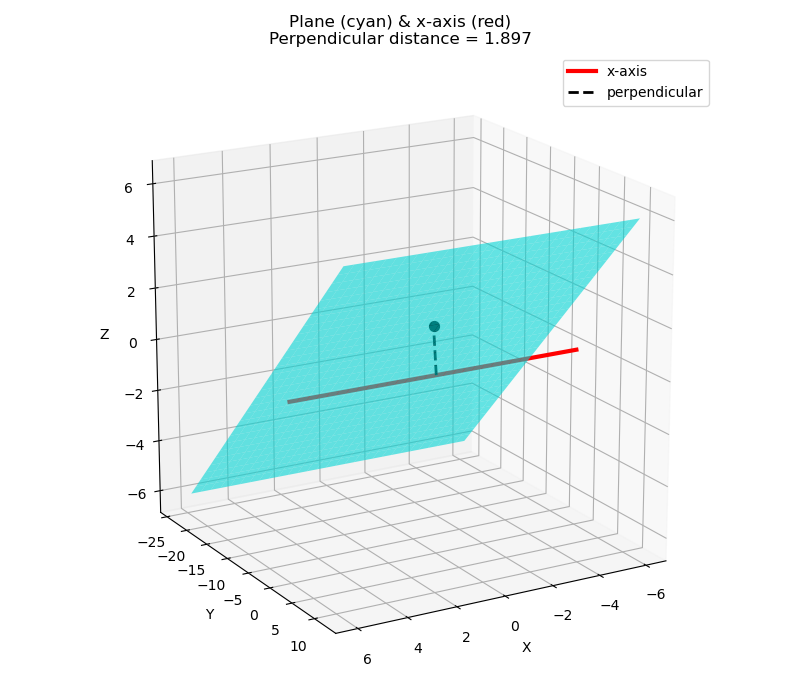
\includegraphics[width=0.7\columnwidth]{figs/plane.png}
   \caption{}
   \label{}
   \end{figure}
\end{frame}

\begin{frame}[fragile]
    \frametitle{Code - C}
    \begin{lstlisting}
#include <stdio.h>
#include <math.h>

// dot product
double dot(const double *a, const double *b, int n) {
    double s = 0.0;
    for (int i = 0; i < n; i++) s += a[i] * b[i];
    return s;
}

// compute n = n1 + k n2
void compute_n(const double *n1, const double *n2, double k, double *res, int n) {
    for (int i = 0; i < n; i++) res[i] = n1[i] + k*n2[i];
}
    \end{lstlisting}
    \end{frame}

    \begin{frame}[fragile]
    \frametitle{Code - C}
    \begin{lstlisting}
// compute constant C = c1 + k c2
double compute_C(double c1, double c2, double k) {
    return c1 + k*c2;
}

// compute k = -(ex.n1)/(ex.n2)
double find_k(const double *ex, const double *n1, const double *n2, int n) {
    double num = dot(ex,n1,n);
    double den = dot(ex,n2,n);
    return -num/den;
}

// norm of vector
double norm(const double *a, int n) {
    return sqrt(dot(a,a,n));
}

\end{lstlisting}
\end{frame}

    \begin{frame}[fragile]
    \frametitle{Code - C}
    \begin{lstlisting}
// distance = |C| / ||n||
double plane_distance(const double *n, double C, int nlen) {
    return fabs(C)/norm(n,nlen);
}

// foot of perpendicular from origin to plane: (C/||n||^2) * n
void foot_point(const double *n, double C, double *res, int nlen) {
    double factor = C/dot(n,n,nlen);
    for (int i = 0; i < nlen; i++) res[i] = factor*n[i];
}


\end{lstlisting}
\end{frame}

\begin{frame}[fragile]
    \frametitle{Code - Python(with shared C code)}
    The code to obtain the required plot is
    \begin{lstlisting}
import ctypes
import numpy as np
import matplotlib.pyplot as plt

# --- load shared library ---
lib = ctypes.CDLL("./libplane3d.so")

# define argtypes/restypes
lib.find_k.restype = ctypes.c_double
lib.find_k.argtypes = [ctypes.POINTER(ctypes.c_double),
                       ctypes.POINTER(ctypes.c_double),
                       ctypes.POINTER(ctypes.c_double),
                       ctypes.c_int]


\end{lstlisting}
\end{frame}
\begin{frame}[fragile]
\frametitle{Code - Python(with shared C code)}
\begin{lstlisting}
lib.compute_n.argtypes = [ctypes.POINTER(ctypes.c_double),
                          ctypes.POINTER(ctypes.c_double),
                          ctypes.c_double,
                          ctypes.POINTER(ctypes.c_double),
                          ctypes.c_int]

lib.compute_C.restype = ctypes.c_double
lib.compute_C.argtypes = [ctypes.c_double, ctypes.c_double, ctypes.c_double]

lib.plane_distance.restype = ctypes.c_double
lib.plane_distance.argtypes = [ctypes.POINTER(ctypes.c_double), ctypes.c_double, ctypes.c_int]

\end{lstlisting}
\end{frame}

\begin{frame}[fragile]
\frametitle{Code - Python(with shared C code)}
\begin{lstlisting}
lib.foot_point.argtypes = [ctypes.POINTER(ctypes.c_double), ctypes.c_double,
                           ctypes.POINTER(ctypes.c_double), ctypes.c_int]

# helper to convert numpy to C array
def c_arr(arr):
    return (ctypes.c_double * len(arr))(*arr.tolist())

# --- input data ---
n1 = np.array([1.0,1.0,1.0])
n2 = np.array([2.0,3.0,-1.0])
c1, c2 = 1.0, -4.0
ex = np.array([1.0,0.0,0.0])

n1_c, n2_c, ex_c = c_arr(n1), c_arr(n2), c_arr(ex)

\end{lstlisting}
\end{frame}

\begin{frame}[fragile]
\frametitle{Code - Python(with shared C code)}
\begin{lstlisting}
# Step 1: find k
k = lib.find_k(ex_c, n1_c, n2_c, 3)

# Step 2: compute plane normal n = n1 + k n2
n_c = (ctypes.c_double * 3)()
lib.compute_n(n1_c, n2_c, ctypes.c_double(k), n_c, 3)
n = np.array([n_c[i] for i in range(3)])

# Step 3: compute constant C
C = lib.compute_C(c1, c2, k)

# Step 4: distance
dist = lib.plane_distance(n_c, C, 3)
\end{lstlisting}
\end{frame}

\begin{frame}[fragile]
\frametitle{Code - Python(with shared C code)}
\begin{lstlisting}
# Step 5: foot of perpendicular from origin to plane
foot_c = (ctypes.c_double * 3)()
lib.foot_point(n_c, C, foot_c, 3)
foot = np.array([foot_c[i] for i in range(3)])

print("k =", k)
print("plane normal n =", n)
print("C =", C)
print("distance =", dist)
print("foot of perpendicular =", foot)

# --- Plotting ---
fig = plt.figure(figsize=(8,7))
ax = fig.add_subplot(111, projection='3d')

\end{lstlisting}
\end{frame}

\begin{frame}[fragile]
\frametitle{Code - Python(with shared C code)}
\begin{lstlisting}
# x-axis
x_line = np.linspace(-6,6,50)
ax.plot(x_line, np.zeros_like(x_line), np.zeros_like(x_line), color='r', lw=3, label="x-axis")

# plane surface
xx, zz = np.meshgrid(np.linspace(-6,6,30), np.linspace(-6,6,30))
yy = (C - n[0]*xx - n[2]*zz)/n[1]
ax.plot_surface(xx,yy,zz,alpha=0.6,color='cyan')

# perpendicular
ax.plot([0, foot[0]], [0, foot[1]], [0, foot[2]], 'k--', lw=2, label="perpendicular")
ax.scatter(*foot, color='k', s=50)

\end{lstlisting}
\end{frame}

\begin{frame}[fragile]
\frametitle{Code - Python(with shared C code)}
\begin{lstlisting}
# labels & view
ax.set_xlabel("X")
ax.set_ylabel("Y")
ax.set_zlabel("Z")
ax.set_title(f"Plane (cyan) & x-axis (red)\nPerpendicular distance = {dist:.3f}")
ax.legend()
ax.view_init(elev=18, azim=60)
ax.set_box_aspect([1,1,1])

plt.tight_layout()
plt.savefig("plane.png")
plt.show()


\end{lstlisting}
\end{frame}


\begin{frame}[fragile]
\frametitle{Code - Python only}
\begin{lstlisting}
import numpy as np
import matplotlib.pyplot as plt

# --- Input data ---
n1 = np.array([1.0, 1.0, 1.0])
n2 = np.array([2.0, 3.0, -1.0])
c1, c2 = 1.0, -4.0
ex = np.array([1.0, 0.0, 0.0])   # x-axis direction

# --- Step 1: find k ---
k = -np.dot(ex, n1) / np.dot(ex, n2)

# --- Step 2: compute plane normal and constant ---
n = n1 + k*n2
C = c1 + k*c2

\end{lstlisting}
\end{frame}
\begin{frame}[fragile]
\frametitle{Code - Python only}
\begin{lstlisting}
# --- Step 3: distance formula ---
dist = abs(C)/np.linalg.norm(n)

# --- Step 4: foot of perpendicular from origin to plane ---
foot = (C/np.dot(n, n)) * n

print("k =", k)
print("plane normal =", n)
print("C =", C)
print("distance from x-axis =", dist)
print("foot of perpendicular =", foot)

# --- Plotting ---
fig = plt.figure(figsize=(8,7))
ax = fig.add_subplot(111, projection='3d')
\end{lstlisting}
\end{frame}

\begin{frame}[fragile]
\frametitle{Code - Python only}
\begin{lstlisting}
# Plot the x-axis (red line)
x_line = np.linspace(-6,6,50)
ax.plot(x_line, np.zeros_like(x_line), np.zeros_like(x_line),
        color='r', lw=3, label="x-axis")

# Plot the plane (cyan surface)
xx, zz = np.meshgrid(np.linspace(-6,6,30), np.linspace(-6,6,30))
yy = (C - n[0]*xx - n[2]*zz)/n[1]
ax.plot_surface(xx, yy, zz, alpha=0.6, color='cyan')

# Plot perpendicular line (black dashed) and foot point (black dot)
ax.plot([0, foot[0]], [0, foot[1]], [0, foot[2]], 'k--', lw=2, label="perpendicular")
ax.scatter(*foot, color='k', s=50)



\end{lstlisting}
\end{frame}

\begin{frame}[fragile]
\frametitle{Code - Python only}
\begin{lstlisting}
# Styling
ax.set_xlabel("X")
ax.set_ylabel("Y")
ax.set_zlabel("Z")
ax.set_title(f"Plane (cyan) & x-axis (red)\nPerpendicular distance = {dist:.3f}")
ax.legend()
ax.view_init(elev=18, azim=60)
ax.set_box_aspect([1,1,1])  # equal aspect ratio

plt.tight_layout()
plt.savefig("new_plane.png")
plt.show()

\end{lstlisting}
\end{frame}

\end{document}